% Created by tikzDevice version 0.12.6 on 2024-10-07 17:49:27
% !TEX encoding = UTF-8 Unicode
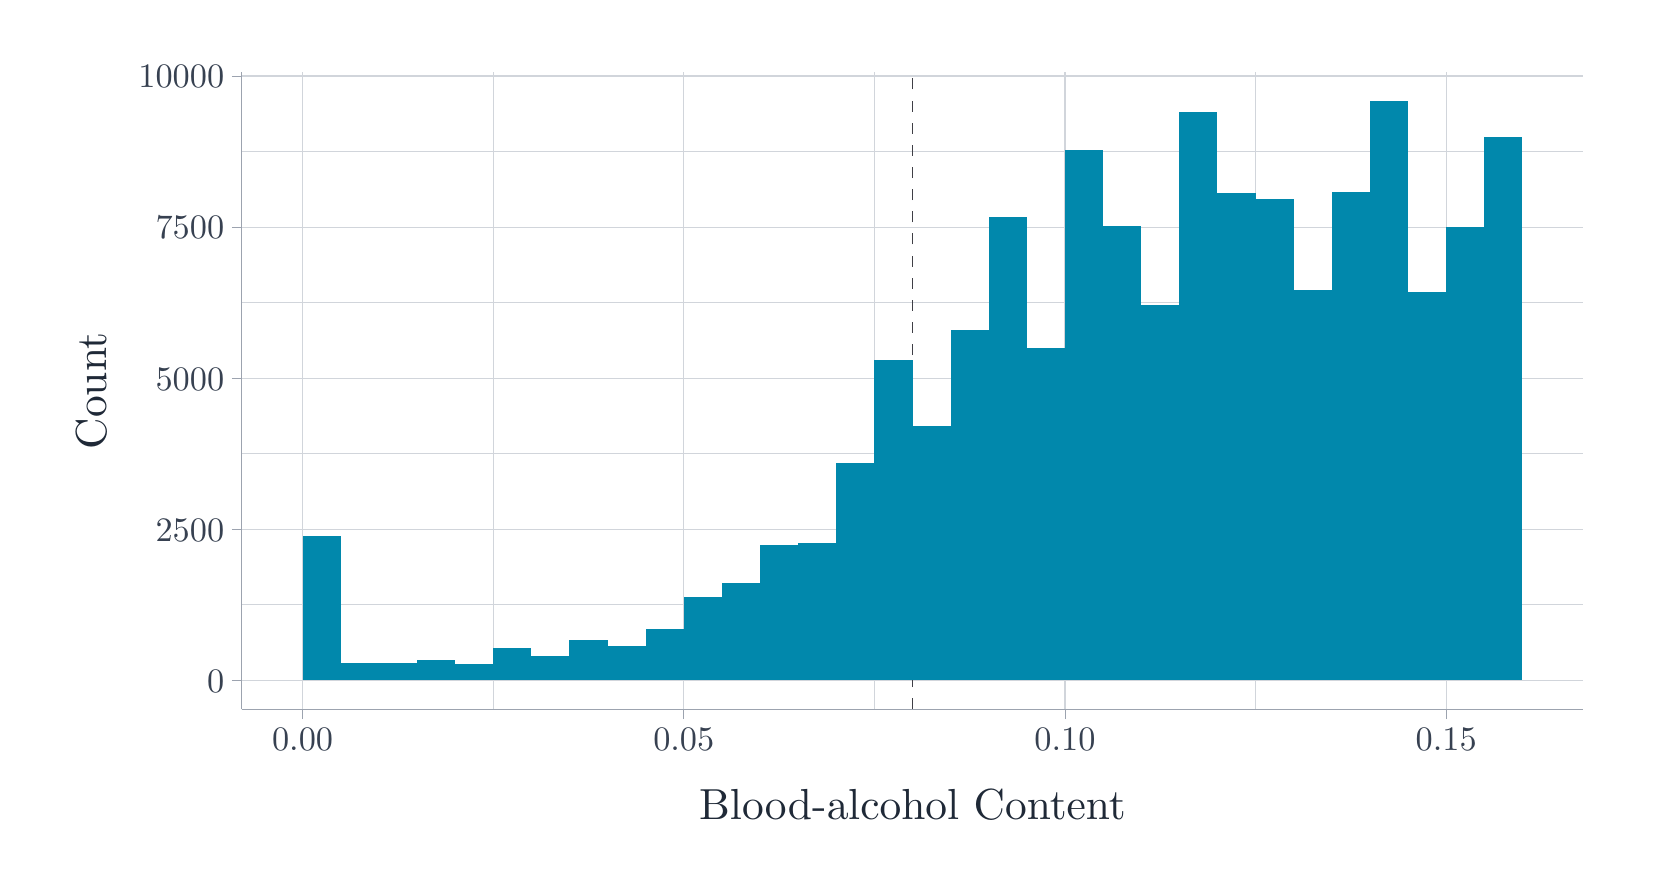
\begin{tikzpicture}[x=1pt,y=1pt]
\definecolor{fillColor}{RGB}{255,255,255}
\path[use as bounding box,fill=fillColor] (0,0) rectangle (578.16,303.53);
\begin{scope}
\path[clip] (  0.00,  0.00) rectangle (578.16,303.53);
\definecolor{drawColor}{RGB}{255,255,255}

\path[draw=drawColor,line width= 0.7pt,line join=round,line cap=round,fill=fillColor] (  0.00,  0.00) rectangle (578.16,303.53);
\end{scope}
\begin{scope}
\path[clip] ( 77.30, 57.20) rectangle (562.16,287.53);
\definecolor{drawColor}{RGB}{255,255,255}
\definecolor{fillColor}{RGB}{255,255,255}

\path[draw=drawColor,line width= 0.7pt,line join=round,line cap=round,fill=fillColor] ( 77.30, 57.20) rectangle (562.16,287.53);
\definecolor{drawColor}{RGB}{209,213,219}

\path[draw=drawColor,line width= 0.4pt,line join=round] ( 77.30, 94.97) --
	(562.16, 94.97);

\path[draw=drawColor,line width= 0.4pt,line join=round] ( 77.30,149.57) --
	(562.16,149.57);

\path[draw=drawColor,line width= 0.4pt,line join=round] ( 77.30,204.18) --
	(562.16,204.18);

\path[draw=drawColor,line width= 0.4pt,line join=round] ( 77.30,258.78) --
	(562.16,258.78);

\path[draw=drawColor,line width= 0.4pt,line join=round] (168.21, 57.20) --
	(168.21,287.53);

\path[draw=drawColor,line width= 0.4pt,line join=round] (305.96, 57.20) --
	(305.96,287.53);

\path[draw=drawColor,line width= 0.4pt,line join=round] (443.70, 57.20) --
	(443.70,287.53);

\path[draw=drawColor,line width= 0.4pt,line join=round] ( 77.30, 67.67) --
	(562.16, 67.67);

\path[draw=drawColor,line width= 0.4pt,line join=round] ( 77.30,122.27) --
	(562.16,122.27);

\path[draw=drawColor,line width= 0.4pt,line join=round] ( 77.30,176.87) --
	(562.16,176.87);

\path[draw=drawColor,line width= 0.4pt,line join=round] ( 77.30,231.48) --
	(562.16,231.48);

\path[draw=drawColor,line width= 0.4pt,line join=round] ( 77.30,286.08) --
	(562.16,286.08);

\path[draw=drawColor,line width= 0.4pt,line join=round] ( 99.34, 57.20) --
	( 99.34,287.53);

\path[draw=drawColor,line width= 0.4pt,line join=round] (237.08, 57.20) --
	(237.08,287.53);

\path[draw=drawColor,line width= 0.4pt,line join=round] (374.83, 57.20) --
	(374.83,287.53);

\path[draw=drawColor,line width= 0.4pt,line join=round] (512.57, 57.20) --
	(512.57,287.53);
\definecolor{drawColor}{RGB}{63,63,70}

\path[draw=drawColor,line width= 0.6pt,dash pattern=on 4pt off 4pt ,line join=round] (319.73, 57.20) -- (319.73,287.53);
\definecolor{fillColor}{RGB}{1,136,172}

\path[fill=fillColor] ( 99.34, 67.67) rectangle (113.11,119.69);

\path[fill=fillColor] (113.11, 67.67) rectangle (126.89, 74.09);

\path[fill=fillColor] (126.89, 67.67) rectangle (140.66, 73.96);

\path[fill=fillColor] (140.66, 67.67) rectangle (154.44, 74.92);

\path[fill=fillColor] (154.44, 67.67) rectangle (168.21, 73.76);

\path[fill=fillColor] (168.21, 67.67) rectangle (181.99, 79.53);

\path[fill=fillColor] (181.99, 67.67) rectangle (195.76, 76.40);

\path[fill=fillColor] (195.76, 67.67) rectangle (209.54, 82.23);

\path[fill=fillColor] (209.54, 67.67) rectangle (223.31, 80.27);

\path[fill=fillColor] (223.31, 67.67) rectangle (237.08, 86.21);

\path[fill=fillColor] (237.08, 67.67) rectangle (250.86, 97.83);

\path[fill=fillColor] (250.86, 67.67) rectangle (264.63,102.83);

\path[fill=fillColor] (264.63, 67.67) rectangle (278.41,116.66);

\path[fill=fillColor] (278.41, 67.67) rectangle (292.18,117.25);

\path[fill=fillColor] (292.18, 67.67) rectangle (305.96,146.14);

\path[fill=fillColor] (305.96, 67.67) rectangle (319.73,183.47);

\path[fill=fillColor] (319.73, 67.67) rectangle (333.51,159.66);

\path[fill=fillColor] (333.51, 67.67) rectangle (347.28,194.13);

\path[fill=fillColor] (347.28, 67.67) rectangle (361.05,235.28);

\path[fill=fillColor] (361.05, 67.67) rectangle (374.83,187.60);

\path[fill=fillColor] (374.83, 67.67) rectangle (388.60,259.26);

\path[fill=fillColor] (388.60, 67.67) rectangle (402.38,231.70);

\path[fill=fillColor] (402.38, 67.67) rectangle (416.15,203.17);

\path[fill=fillColor] (416.15, 67.67) rectangle (429.93,273.02);

\path[fill=fillColor] (429.93, 67.67) rectangle (443.70,243.80);

\path[fill=fillColor] (443.70, 67.67) rectangle (457.47,241.44);

\path[fill=fillColor] (457.47, 67.67) rectangle (471.25,208.85);

\path[fill=fillColor] (471.25, 67.67) rectangle (485.02,244.28);

\path[fill=fillColor] (485.02, 67.67) rectangle (498.80,277.06);

\path[fill=fillColor] (498.80, 67.67) rectangle (512.57,207.89);

\path[fill=fillColor] (512.57, 67.67) rectangle (526.35,231.48);

\path[fill=fillColor] (526.35, 67.67) rectangle (540.12,264.00);
\end{scope}
\begin{scope}
\path[clip] (  0.00,  0.00) rectangle (578.16,303.53);
\definecolor{drawColor}{RGB}{156,163,175}

\path[draw=drawColor,line width= 0.3pt,line join=round] ( 77.30, 57.20) --
	( 77.30,287.53);
\end{scope}
\begin{scope}
\path[clip] (  0.00,  0.00) rectangle (578.16,303.53);
\definecolor{drawColor}{RGB}{55,65,81}

\node[text=drawColor,anchor=base east,inner sep=0pt, outer sep=0pt, scale=  1.24] at ( 71.00, 63.38) {0};

\node[text=drawColor,anchor=base east,inner sep=0pt, outer sep=0pt, scale=  1.24] at ( 71.00,117.99) {2500};

\node[text=drawColor,anchor=base east,inner sep=0pt, outer sep=0pt, scale=  1.24] at ( 71.00,172.59) {5000};

\node[text=drawColor,anchor=base east,inner sep=0pt, outer sep=0pt, scale=  1.24] at ( 71.00,227.20) {7500};

\node[text=drawColor,anchor=base east,inner sep=0pt, outer sep=0pt, scale=  1.24] at ( 71.00,281.80) {10000};
\end{scope}
\begin{scope}
\path[clip] (  0.00,  0.00) rectangle (578.16,303.53);
\definecolor{drawColor}{RGB}{156,163,175}

\path[draw=drawColor,line width= 0.3pt,line join=round] ( 73.80, 67.67) --
	( 77.30, 67.67);

\path[draw=drawColor,line width= 0.3pt,line join=round] ( 73.80,122.27) --
	( 77.30,122.27);

\path[draw=drawColor,line width= 0.3pt,line join=round] ( 73.80,176.87) --
	( 77.30,176.87);

\path[draw=drawColor,line width= 0.3pt,line join=round] ( 73.80,231.48) --
	( 77.30,231.48);

\path[draw=drawColor,line width= 0.3pt,line join=round] ( 73.80,286.08) --
	( 77.30,286.08);
\end{scope}
\begin{scope}
\path[clip] (  0.00,  0.00) rectangle (578.16,303.53);
\definecolor{drawColor}{RGB}{156,163,175}

\path[draw=drawColor,line width= 0.3pt,line join=round] ( 77.30, 57.20) --
	(562.16, 57.20);
\end{scope}
\begin{scope}
\path[clip] (  0.00,  0.00) rectangle (578.16,303.53);
\definecolor{drawColor}{RGB}{156,163,175}

\path[draw=drawColor,line width= 0.3pt,line join=round] ( 99.34, 53.70) --
	( 99.34, 57.20);

\path[draw=drawColor,line width= 0.3pt,line join=round] (237.08, 53.70) --
	(237.08, 57.20);

\path[draw=drawColor,line width= 0.3pt,line join=round] (374.83, 53.70) --
	(374.83, 57.20);

\path[draw=drawColor,line width= 0.3pt,line join=round] (512.57, 53.70) --
	(512.57, 57.20);
\end{scope}
\begin{scope}
\path[clip] (  0.00,  0.00) rectangle (578.16,303.53);
\definecolor{drawColor}{RGB}{55,65,81}

\node[text=drawColor,anchor=base,inner sep=0pt, outer sep=0pt, scale=  1.24] at ( 99.34, 42.33) {0.00};

\node[text=drawColor,anchor=base,inner sep=0pt, outer sep=0pt, scale=  1.24] at (237.08, 42.33) {0.05};

\node[text=drawColor,anchor=base,inner sep=0pt, outer sep=0pt, scale=  1.24] at (374.83, 42.33) {0.10};

\node[text=drawColor,anchor=base,inner sep=0pt, outer sep=0pt, scale=  1.24] at (512.57, 42.33) {0.15};
\end{scope}
\begin{scope}
\path[clip] (  0.00,  0.00) rectangle (578.16,303.53);
\definecolor{drawColor}{RGB}{31,41,55}

\node[text=drawColor,anchor=base,inner sep=0pt, outer sep=0pt, scale=  1.57] at (319.73, 17.53) {Blood-alcohol Content};
\end{scope}
\begin{scope}
\path[clip] (  0.00,  0.00) rectangle (578.16,303.53);
\definecolor{drawColor}{RGB}{31,41,55}

\node[text=drawColor,rotate= 90.00,anchor=base,inner sep=0pt, outer sep=0pt, scale=  1.57] at ( 28.38,172.36) {Count};
\end{scope}
\end{tikzpicture}
